\scanpage{47}
\mspage{3)}

qui forment un groupoïde \deleted{\unsure{$MD$}}. $\mathrm{Grbip}$ \deleted{\unsure{ou}} $(\mathrm{Grabipond})$

Objets : graphes \inserted{finis} $(S,\vec A,\sigma,o)$ \inserted{$+$ structure suppl.} (pouvant avoir des sommets isolés, des boucles fermées, a fortiori plusieurs arêtes entre deux sommets, et aussi des ``\uline{arêtes libres}'' correspondant aux pts fixes de $\sigma$)

% slanted
\margin{pas assez \unsure{précis|précisé} comme donnée. --- La pondération d'une arête doit être remplacée par celle d'un pol. comb. $T_a$ avec $\unsure{\omega(T_a)\simeq a|\mathrm{or}(T_a)\simeq a|n(T_a)\simeq a}$.}

$S,\vec A$ ens. finis \inserted{(``sommets'', ``arcs'')}, $\sigma:\vec A\unsure{-|\to}\vec A$ involution, $o:\vec A\to S$ appl\textsuperscript{n} ``origine''. On se donne de plus

\margin{J'ai indiqué une pondération des sommets, mais pas des arêtes}

\figure{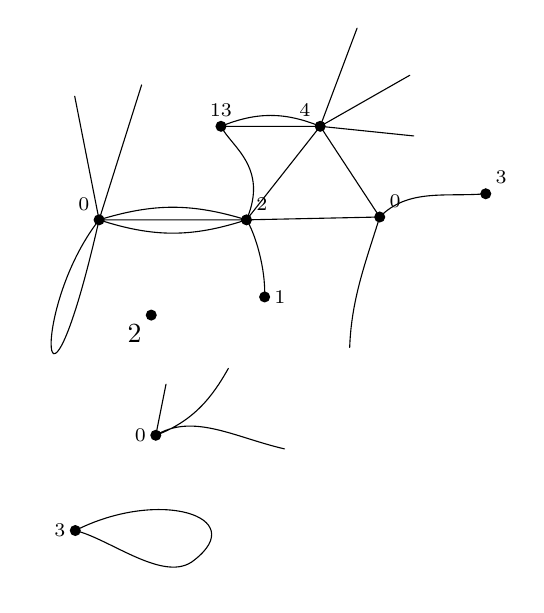
\begin{tikzpicture}[x=.72cm,y=.72cm,line cap=round]
\coordinate (a) at (0,2); \coordinate (b) at (2.6,2); \coordinate (c) at (2.15,3.65);
\coordinate (d) at (3.9,3.65); \coordinate (e) at (4.95,2.05);
\draw (a) to[bend left=17] (b) (a)--(b) (a) to[bend right=18] (b);
\draw (a) .. controls (-1.25,.4) and (-1.0,-2.4) .. (a);
\draw (a)--(-.43,4.18) (a)--(.75,4.38);
\draw (b) .. controls (3.0,2.93) and (2.32,3.3) .. (c);
\draw (c)--(d) (c) to[bend left=22] (d) (b)--(d)--(e)--(b);
\draw (d)--(4.55,5.38) (d)--(5.48,4.55) (d)--(5.55,3.48);
\draw (e).. controls (4.7,1.25) and (4.45,.6) ..(4.42,-.25);
\draw (e).. controls (5.45,2.56) and (6.12,2.4) ..(6.82,2.46);
\draw (b) .. controls (2.75,1.77) and (2.94,1.15) ..(2.92,.64);
\foreach \p/\lab/\where in {a/0/above left,b/2/above right,c/13/above,d/4/above left,e/0/above right}
 {\fill (\p) circle (2pt) node[\where] {\scriptsize $\lab$};}
\fill (6.82,2.46) circle (2pt) node[above right]{\scriptsize $3$};
\fill (2.92,.64) circle (2pt) node[right]{\scriptsize $1$};
\fill (.92,.32) circle (2pt) node[below left]{$2$};
\draw (1,-1.8)--(1.18,-.9) (1,-1.8) .. controls (1.67,-1.55) and (2,-1.12) ..(2.28,-.62)
 (1,-1.8).. controls (1.66,-1.4) and (2.4,-1.84) ..(3.27,-2.04);
\fill (1,-1.8) circle (2pt) node[left]{\scriptsize $0$};
\draw (-.42,-3.48) .. controls (1.06,-2.73) and (2.67,-3.23) ..(1.68,-4.0) .. controls (1.17,-4.43) and (.2,-3.63) ..(-.42,-3.48);
\fill (-.42,-3.48) circle (2pt) node[left]{\scriptsize $3$};
\end{tikzpicture}}

\[
 S\xrightarrow{\deleted{\unsure{g}}\gamma}\mathbb N\qquad\text{(application ``genre'' ou ``poids'')}
\]

\[
 \deleted{\unsure{\vec A^{\sigma}}=}\widetilde A \xrightarrow{r\,\deleted{\unsure{\rho_2|\rho z}}}\mathbb N
 \qquad\text{(application \deleted{\unsure{rigi}}\deleted{\unsure{de marquage et}} ``indice de rigidification'')}
\]
\deleted{``\unsure{ensemble des arêtes libres}''}
\[
 \widetilde A\overset{\text{déf}}{=}\vec A/\sigma
\]

\deleted{Ou encore, posant $\widetilde S=S\amalg A_l$, (identifié à l'ens. de \uline{tous} les ``sommets'', \inserted{apparents} \deleted{\unsure{marqués}} et \uline{``masqués''} (i.e. $\unsure{\in S|\notin S}$) \inserted{et fictifs (ces d. correspondant aux $\in A_l$)} du graphe), on donne}
\[
 \deleted{\widetilde S\xrightarrow{\pi}\mathbb N}\qquad\text{(\uline{pondération} du graphe)}
\]
\deleted{``\unsure{ens. des sommets apparents}''}

\margin{$\widetilde S=S\amalg\deleted{\unsure{S_l}}{}\underset{\shortparallel}{\unsure{S_l}}$ \deleted{\unsure{sommets fictifs}}\\ $A_l$}

La donnée du \uline{graphe} sous-jacent à un graphe \deleted{$MD$} \inserted{bip.} revient à celle du graphe ``ordinaire'' correspondant (sans arêtes \uline{libres}, i.e. où $\sigma$ opère sans pts fixes), i.e.
\[
 (S,(\vec A\setminus\vec A^\sigma),\sigma|(\vec A\setminus\vec A^\sigma),o|{\vec A\setminus\vec A^\sigma}),
\]
\uline{plus} un ensemble \inserted{fini} $A_l$ (\deleted{\unsure{sommets}} \inserted{arêtes} libres) \deleted{ou ``sommets-trous'')} et une application
\[
 A_l\longrightarrow S
\]

\margin{$\widetilde A=\vec A/\sigma=A\amalg A_l$}

\diagram{\begin{tikzcd}[ampersand replacement=\&,row sep=large,column sep=small]
\vec A \arrow[d]\arrow[d,shift right=1.5,no head,"\deleted{\unsure{\pi}}"'] \& {}={} \&
\underbrace{\vec A_{0}}_{\vec A\setminus\vec A^\sigma}\arrow[d,"\mathrm{deg}\,2"]
 \& {}\amalg{} \& \underbrace{\vec A_l}_{\vec A^\sigma}\arrow[d,"\mathrm{deg}\,1"]\\
\widetilde A \& {}={} \& A \& {}\amalg{} \& A_l
\end{tikzcd}}

\margin{Ordre d'un sommet\\ $\sigma(s)=\underbrace{\sigma_l(s)}_{\substack{\text{correspond}\\\text{aux ``trous''}\\\text{ou cercles}\\\text{de recollage}}}+\sigma_{\unsure{0|o}}(s)$}

\uline{Flèches} \qquad les iso. de telles structures
% archive sheet number: 46

